\chapter{Útkereső algoritmus}

A későbbiekben bemutatásra kerülő generálási módokhoz szükséges áttekinteni az útkereső algoritmusok témakörét. A hexagonokból és a négyzetekből felépülő rácsok esetében az útvonalkeresés alapvetően ugyanúgy működik. Lényegi különbség a cellák szomszédos elemeinek számában van, így elegendő az útvonakeresést csak a négyzetrács esetében megvizsgálni.

\section{Algoritmusok}
\cite{algoritmusok}
\cite{redblobA*}
\cite{Dijkstra}
\cite{Pathfinding}
\cite{A*}
\cite{Breadth-first_search}

A kereső algoritmusokat két pont közötti út megtalálására alkalmazzuk. 
A kereső algoritmusoknak több fajtája van, ezek különbözőképpen közelítik meg a problémát. 
\begin{itemize}
\item Az egyik csoport minden esetben talál egy megoldást ami nem feltétlenül a legrövidebb út viszont egy elfogadható közelítése annak (\textit{A algoritmusok}). Ezek az algoritmusok széleskörűen alkalmazhatóak ellentétben a másik csoporttal, mivel azok csak speciális esetekben használhatóak, mivel ezekhez további információk szükségesek a gráfról, amik nem minden esetben állnak rendelkezésünkre.
\item A másik csoport ami minden esetben az optimális útvonalat találja meg, ha az létezik (\textit{A*-algoritmus}).
\end{itemize}

Az általános algoritmusok úgy keresik a megoldást, hogy a kezdő ponttól kiindulva végignézik a szomszédos csomópontokat és ezt ismétlik mindaddig, amíg meg nem találják a végpontot. Az általános algoritmusok, mint például a \textit{szélességi keresés} algoritmus is megtalálja az útvonalat ha megadjuk az ehhez szükséges időt, viszont olyan megoldások amik ,,ismerik'' a gráfot általánosságban hamarabb elérik a célt.

Két problémát kell megoldanunk az útkereséssel kapcsolatban: 
\begin{itemize}
\item első az útvonal megtalálása két pont között, 
\item a második az, hogy a legrövidebb utat találjuk meg. 
\end{itemize}

Olyan alapvető algoritmusok, mint a \textit{szélességi
keresés} vagy a \textit{mélységi keresés} nagyon egyszerűen megoldják az első problémánkat azáltal, hogy az összes lehetséges útvonalat bejárják. Ezek az algoritmusok $\mathcal{O}(|V| + |E|)$ (lineáris) futásidejűek, ahol $V$ a csúcsok száma és $E$ az élek száma.

A legrövidebb út megtalálása már ennél jóval komplexebb probléma. Edsger Dijkstra találta meg erre a problémára a megoldást 1956-ban \cite{Dijkstra}. Az algoritmusából manapság már több változat is létezik. Dijkstra eredeti algoritmusa megtalálta a legrövidebb utat két csúcs között egy súlyozott gráfon, de manapság a leggyakoribb változata úgy változtatja meg az algoritmust, hogy egy megadott csúcsponthoz viszonyítva kiszámítja az összes többi csúcsponthoz vezető legrövidebb utat, ezáltal előállítva a legrövidebb út fát. Ennek a futásideje $\mathcal{O}(|E| + |V| log|V|)$.

A \textit{Bellman-Ford} algoritmus ugyanazt a problémát oldja meg mint a \textit{Dijkstra algoritmus}, viszont ez egy sokoldalúbb algoritmus, mivel az élek értéke negatív értéket is felvehet \cite{bellman}. Mindössze azt kell kizárni, hogy a gráf negatív összköltségű kört tartalmazzon. Negatív költségű él például úgy keletkezhet, hogy nagyobb bevételhez jutunk azon a szakaszon mint amennyi ráfordítással jár. A legrosszabb esetű futásideje $\mathcal{O}(|V||E|)$, de bizonyos esetekben akár $\mathcal{O}(|V|)$ is lehet, ami azt jelenti, hogy legrosszabb esetben lassabb mint a \textit{Dijkstra-féle algoritmus}.

Általában nem szükséges az összes lehetséges útvonalat bejárni ahhoz, hogy megtaláljuk az optimális útvonalat. Olyan algoritmusok, mint a \textit{Dijkstra} vagy az \textit{A*} algoritmus heurisztikák segítségével eliminálja az olyan útvonalakat amik nem lehetségesek vagy nem vezetnek a megoldás felé. Ezáltal el tudják érni az $\mathcal{O}(|E| log(|V|))$ futásidőt. 

A fent említett algoritmusok a legjobb általános algoritmusok közé tartoznak amikkel előfeldolgozás nélkül is ki lehet értékelni egy gráfot. Gyakorlatban elérhető még ezeknél is jobb idő komplexitású algoritmus, ha előfeldolgozzuk a gráfot.

A következő szakaszokban ismeretésre kerülnek a leggyakrabban alkalmazott algoritmusok.

\subsection{A szélességi keresés algoritmusa}
\cite{algoritmusok}
\cite{Pathfinding}
\cite{Breadth-first_search}

A \textit{szélességi keresés} (\textit{breadth-first search}) egy egyszerűnek számító keresési algoritmus (\ref{fig:breadth-first_search}. ábra). A térképen minden egyes irányban egységes mértékben keres. Ez egy teljes keresés, ezáltal minden esetben a legrövidebb utat fogja megtalálni a célhoz. A keresés a gyökér csomóponttól indul és úgy folytatódik, hogy az összes csomópontot kiértékeli ami a gyökér csomópontból elérhető. Ezután ezekből a csomópontokból elérhető csomópontokat értékeli ki. Ez mindig egy adott mélységen lévő csomópontokat értékeli ki egyszerre és ezután halad tovább a következő szintre. Könnyen belátható, hogy az algoritmus a FIFO (first-in-first-out) elv alapján működik. Tehát azokat az elemeket értékeli ki először egy adott listáról amik először felkerültek a listára. Ezáltal belátható, hogy ez az algoritmus a legmagasabb szinten található cél csomópontot fogja megtalálni először. 

\begin{figure}[h!]
\centering
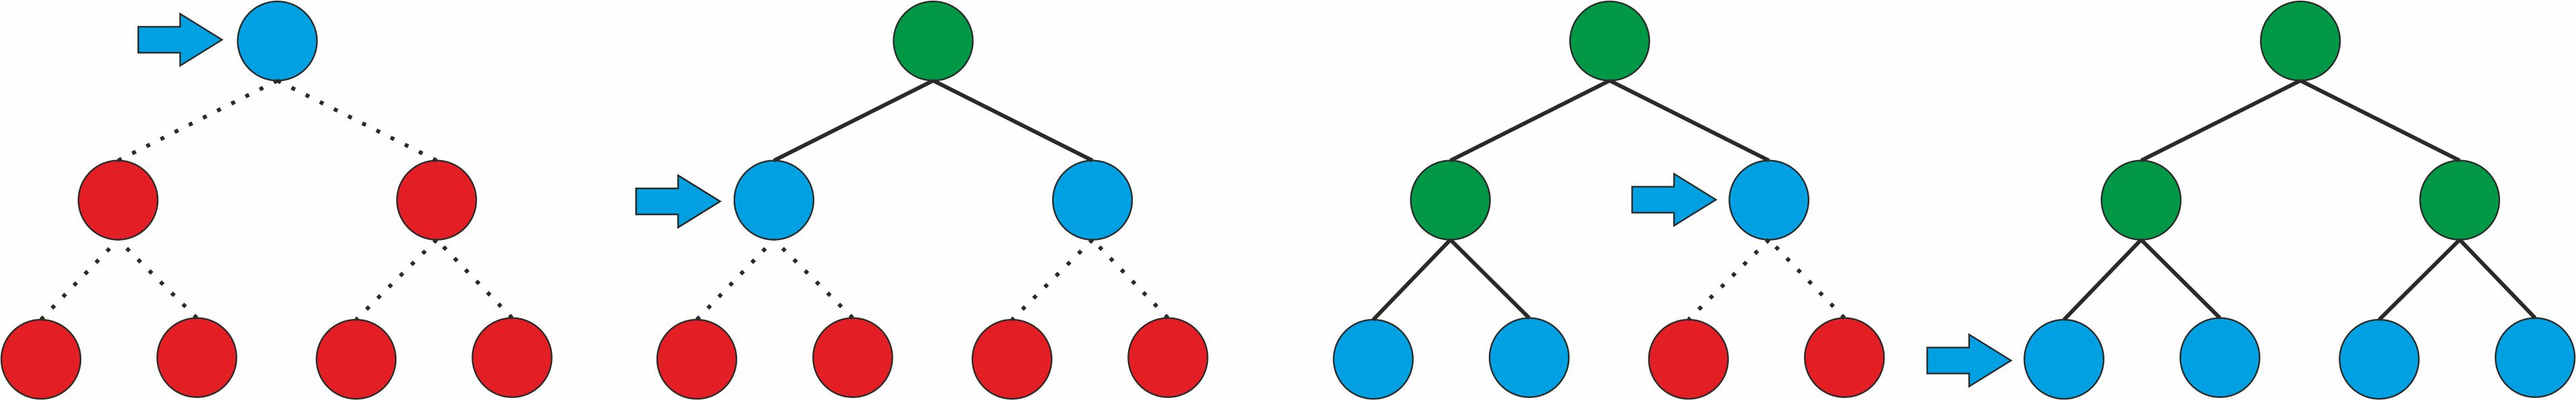
\includegraphics[scale=0.4]{kepek/breadth-first_search.jpg}
\caption{Szélességi keresés algoritmus lépései}
\label{fig:breadth-first_search}
\end{figure}

\newpage
Mivel ez egy teljes keresés, az egész gráf kiértékelésre kerül. Nem feltétlenül a legmagasabban található cél csomóponthoz vezető úton jutunk el a leggyorsabban a célhoz, ha az éleknek különbözik a súlya. Ezért érdemes olyan esetekben használni amikor a gráf éleinek nincs súlya vagy egységes súlyuk van, mert általában elegendő a legmagasabban található cél csomópontig eljutni. Érdemes továbbá tisztázni, hogy ha a térképen egy darab célpontunk van, az a gráfban több célcsomópontként is megjelenhet, mivel a gráf különböző útvonalai a különböző útvonalakat jelölik ugyanazon célhoz, de egyszerre akár több célunk is lehet a térképen.

A \textit{szélességi keresés algoritmus} legnagyobb hátránya a tárigénye. Vegyünk például egy hipotetikus állapotteret, ahol minden kifejtéskor $x$ darab új csomópontot kapunk állapotunk van. Tehát a gyökér kifejtésekor $x$ darab elemünk lesz. Második szinten $x^2$. Tegyük fel, hogy a cél csomópontunk n mélységben található, ekkor legrosszabb esetben $x^n - x$ csomópontot kell kiértékelnünk, mivel az utolsó mélységet már nem szükséges kiértékelnünk. 

A \textit{szélességi keresés algoritmus} egy nem informált keresés mivel a cél csomópontról nem rendelkezik információval. A továbbiakban csak informált keresésekről esik majd szó.

\subsection{Dijkstra algoritmus}
\cite{algoritmusok}
\cite{Dijkstra}
\cite{Pathfinding}

Gyakori példa a gráf alapú útkereső algoritmusra a \textit{Dijkstra algoritmus}. A \textit{szélességi keresés} módszerrel ellentétben nem egységesen fedezi fel az utakat, hanem a kisebb útköltségűeket priorizálja. Ennek az algoritmusnak az elején szükségünk lesz egy kezdő csomópontra és egy listára a ,,nyitott'' csomópontoknak. Ebbe kerülnek azok a csomópontok amiket még ki kell értékelnünk. Minden iterációban az a csomópont kerül kiértékelésre amelyiknek a legkisebb az útköltsége a kezdő csomóponttól mérve. A számítógépes játékok esetében az útköltség függhet például attól, hogy milyen területen haladunk (magassági viszonyok változásától, a talaj anyagától, időjárási viszonyoktól, egyéb környezeti viszonyoktól, ha az úton ellenség van akkor is megnövelhetjük az út költségét). Az algoritmus alapvetően súlyozott élek esetén működik, de használható súlyozatlan élek esetén is, ekkor a súlyozatlan élek értékét válasszuk 1-nek. Akkor kerül egy csomópont ,,lezárásra'', hogy ha már az összes szomszédja hozzá lett adva a nyitott csomópontok listájához, vagy már lezárásra került. Ez a folyamat addig ismétlődik amíg az algoritmus megtalálja az első útvonalat a célhoz (ami lehet akár az összes csomópont is). Mivel mindig a legkisebb útköltségre lévő út fog kiértékelődni, ezért amit először megtalál, az lesz a legrövidebb út. Tehát változatos útköltségek esetén érdemesebb a \textit{Dijkstra algoritmus}t használni a \textit{szélességi keresés} módszer helyett.

\newpage
\subsection{A*-algoritmus}
\cite{algoritmusok}
\cite{redblobA*}
\cite{Pathfinding}
\cite{A*}

Az \textit{A*-algoritmus} a \textit{Dijkstra algoritmus} továbbfejlesztett változata, amit gyorsasága és a pontossága miatt előszeretettel alkalmaznak játékok készítésekor, olyan esetekben, amikor csak egy konkrét célponthoz kell eljutni. A két algoritmus közötti fő különbség abban rejlik, hogy melyik csomópontot választja ki az algoritmus kiértékelésre a nyitott csomópontok közül. Ahhoz, hogy megértsük az \textit{A*} kiválasztási módszerét először meg kell ismernünk 3 fogalmat:
\begin{itemize}
\item \textit{G költség}: Az adott csomóponthoz vezető út költsége a kezdő csomóponthoz képest.
\item \textit{H költség (heurisztikus költség)}: A becsült távolság a célhoz képest.
\item \textit{F költség}: $F = G + H$. Ez az érték alapján kerül kiválasztásra a kiértékelendő csomópont.
\end{itemize}

A \textit{Dijkstra algoritmus}sal ellentétben nem az útköltségek alapján priorizál hanem a célponttól lévő távolság alapján.

A \textit{G költség} tulajdonképpen a \textit{Dijkstra algoritmus} használata, amit az \textit{A*-algo\-rit\-mus} egy heurisztikus költséggel egészít ki, annak érdekében, hogy kizárjuk a hosszabb útvonalakat. Heurisztikaként leggyakrabban a \textit{Manhattan-formulát} szokták használni. Amennyiben a heurisztikus költséget 0-ra ''állítjuk be'', akkor az algoritmus megegyezik a \textit{Dijkstra algoritmus}sal.

Az útkereső algoritmus készítéséhez szükséges ismernünk azt, hogy a térkép egy mezőjéről hogyan érhetőek el a szomszédos mezők és szükséges ismernünk a távolság számító algoritmusokat is. A távolság számító algoritmusok \aref{sec:tavolsag}. szakaszban már ismertetésre kerültek, ezért most vizsgáljuk meg a szomszédok kezelését.

\section{Szomszédok}
\cite{redblobgamesHexagonalGrids}

Ahhoz, hogy útkereső algoritmust tudjunk készíteni ismernünk kell, hogy a különböző alakzatok és koordináta-rendszerek esetén milyen algoritmussal érhetjük el az adott alakzat szomszédait. 

\subsection{Négyzet}
\cite{redblobA*}

Derékszögű, két dimenziós koordináta-rendszer esetén egy adott $(u, v)$ koordinátára eső pont (ahol $u, v \in \mathbb{Z}$) szomszédos pontjait a következő hozzárendeléssel adhatjuk meg:
$$
(u, v) \rightarrow
\left\{
(u, v+1), (u+1, v), (u, v-1), (u-1, v)
\right\}.
$$

Ahogy láthatjuk, a szomszédok koordinátáinak kiszámítása vektorokkal való eltolásokat jelent. A következőkben a példák C\# programozási nyelven szerepelnek, mivel így közvetlenül látszódnak a számítási módjuk, és a matematikai leírásmód sem eredményezne egyszerűbb felírást.

\subsection{Hexagon}

Hexagonok esetén az egyes koordináta-rendszer típusoktól függően különböző módokon tudjuk kiszámítani a szomszédos elemek halmazát.

\subsubsection{Kocka koordináta-rendszer}
\cite{redblobgamesHexagonalGrids}

Ahhoz, hogy elmozduljunk eggyel meg kell változtatnunk egyet a három kocka koordináta közül $+1$-el és egy másikat $-1$-el (a változtatások összege $0$ kell, hogy legyen). Három koordinátát lehet megváltoztatni $+1$-el, a másik két lehetséges koordináta közül az egyiket kell csökkenteni $-1$-el. Ez hat lehetséges változatot eredményez. Mindegyik megfeleltethető a hexagon egyik irányának. A lehető legegyszerűbb és leggyorsabb megoldás az, ha az összes lehetséges permutációt előre kiszámítjuk, és beleírjuk egy tömbbe (\texttt{cubeDirections}). Ezzel az irányok egy $[0, 3]$ közötti egész értékkel (\texttt{direction}) megadhatók.
\begin{cpp}
Cube[] cubeDirections = 
{ 
   Cube(+1, -1,  0), Cube(+1,  0, -1), Cube( 0, +1, -1),
   Cube(-1, +1,  0), Cube(-1,  0, +1), Cube( 0, -1, +1) 
};

public Cube CubeDirection(int direction)
{
   return cubeDirections[direction];
}

public Cube CubeNeighbor(Cube cube, int direction)
{
   return Cube
   (
      cube.x + cubeDirections[direction].x, 
      cube.y + cubeDirections[direction].y, 
      cube.z + cubeDirections[direction].z
   );
}
\end{cpp}

\subsubsection{Tengely koordináta-rendszer}
\cite{redblobgamesHexagonalGrids}

\noindent A \textit{tengely koordináta-rendszer}ben való számításokhoz a \textit{kocka koordináta-rendszer}hez megadott irányokat kell átalakítanunk \textit{tengely koordináta-rendszer}nek megfelelően. A 6 lehetséges irány miatt az egyes irányok egy $[0, 5]$ intervallumon értelmezett indexszel jelölhetők ki.
\begin{cpp}
Axial[] axialDirections = 
{ 
   Axial(+1,  0), Axial(+1, -1), Axial( 0, -1),
   Axial(-1,  0), Axial(-1, +1), Axial( 0, +1)
};

public Axial AxialDirection(int direction)
{
   return axialDirections[direction];
}

public Axial AxialNeighbor(Axial axial, int direction)
{
   return Axial
   (
      axial.x + axialDirections[direction].x, 
      axial.y + axialDirections[direction].y, 
   );
}
\end{cpp}

\subsubsection{Eltolásos koordináta-rendszer}
\cite{redblobgamesHexagonalGrids}

\textit{Eltolásos koordináta-rendszer} esetén a lépések változnak annak a függvényében, hogy hol állunk a hálóban. Ha mi egy eltolt oszlopban/sorban állunk akkor a szabály eltér attól, mint ha egy nem eltolt oszlopban/sorban állnánk.

Ahogy a korábbi esetekben úgy most is kell készítenünk egy táblázatot amiben azt tároljuk majd, hogy a különböző tengelyeken mennyit kell hozzáadni, hogy elérjük a szomszédokat. Ebben az esetben most két tömbre lesz szükségünk, az egyik a páros sor/oszlop a másik pedig a páratlan sor/oszlop esetére.

A táblázat különbözik mind a négy eltolásos módszernél.

\bigskip

Páratlan sor eltolása esetén:
\begin{cpp}
OddRow[,] oddRowDirections = 
{ 
   [ 
      OddRow(+1,  0), OddRow( 0, -1), OddRow(-1, -1),
      OddRow(-1,  0), OddRow(-1, +1), OddRow( 0, +1) 
   ],
   [ 
      OddRow(+1,  0), OddRow(+1, -1), OddRow( 0, -1),
      OddRow(-1,  0), OddRow( 0, +1), OddRow(+1, +1) 
   ]
};

public OddRow OddRowNeighbor(OddRow oddRow, int direction)
{
   int parity = oddRow.row \% 2;
   OddRow dir = oddRowDirections[parity][direction];
   return OddRow(oddRow.col + dir.col, oddRow.row + dir.row);
}   
\end{cpp}

Páros sor eltolása esetén:
\begin{cpp}  
EvenRow[,] evenRowDirections = 
{ 
   [
      EvenRow(+1,  0), EvenRow(+1, -1), EvenRow( 0, -1),
      EvenRow(-1,  0), EvenRow( 0, +1), EvenRow(+1, +1) 
   ],
   [ 
      EvenRow(+1,  0), EvenRow( 0, -1), EvenRow(-1, -1),
      EvenRow(-1,  0), EvenRow(-1, +1), EvenRow( 0, +1) 
   ]
};

public EvenRow EvenRowNeighbor(EvenRow evenRow, int direction)
{
   int parity = evenRow.row \% 2;
   EvenRow dir = evenRowDirections[parity][direction];
   return EvenRow(evenRow.col + dir.col, evenRow.row + dir.row);
}   
\end{cpp}

Páratlan oszlop eltolása esetén:
\begin{cpp}
OddColumn[,] oddColumnDirections = 
{ 
   [ 
      OddColumn(+1,  0), OddColumn(+1, -1), OddColumn( 0, -1),
      OddColumn(-1, -1), OddColumn(-1,  0), OddColumn( 0, +1) 
   ],
   [ 
      OddColumn(+1, +1), OddColumn(+1,  0), OddColumn( 0, -1),
      OddColumn(-1,  0), OddColumn(-1, +1), OddColumn( 0, +1) 
   ]
};

public OddColumn OddColumnNeighbor(OddColumn oddColumn, int direction)
{
   int parity = oddColumn.col \% 2;
   OddColumn dir = oddColumnDirections[parity][direction];
   return OddColumn(oddColumn.col + dir.col, oddColumn.row + dir.row);
}   
\end{cpp}

Páros oszlop eltolása esetén
\begin{cpp}
EvenColumn[,] evenColumnnDirections = 
{ 
   [ 
      EvenColumn(+1, +1), EvenColumn(+1,  0), EvenColumn( 0, -1),
      EvenColumn(-1,  0), EvenColumn(-1, +1), EvenColumn( 0, +1) 
   ],
   [  
      EvenColumn(+1,  0), EvenColumn(+1, -1), EvenColumn( 0, -1),
      EvenColumn(-1, -1), EvenColumn(-1,  0), EvenColumn( 0, +1) 
   ]
};

public EvenColumn EvenColumnNeighbor
(
   EvenColumn evenColumn, 
   int direction
)
{
   int parity = evenColumn.col \% 2;
   EvenColumn dir = evenColumnDirections[parity][direction];
   return EvenColumn(evenColumn.col + dir.col, evenColumn.row + dir.row);
}   
\end{cpp}

\subsubsection{Átlós szomszédok}
\cite{redblobgamesHexagonalGrids}

\noindent Az “átlós” szomszédok a kocka koordináták esetén úgy kerülnek meghatározásra, hogy a lehetséges három koordináta közül az egyiket $ \pm 2$ -vel, míg a másik kettőt $\mp 1$ -el módosítjuk, hogy a három koordináta összege mindig $0$ legyen (\ref{fig:Diagonals}).

\begin{figure}[h!]
\centering
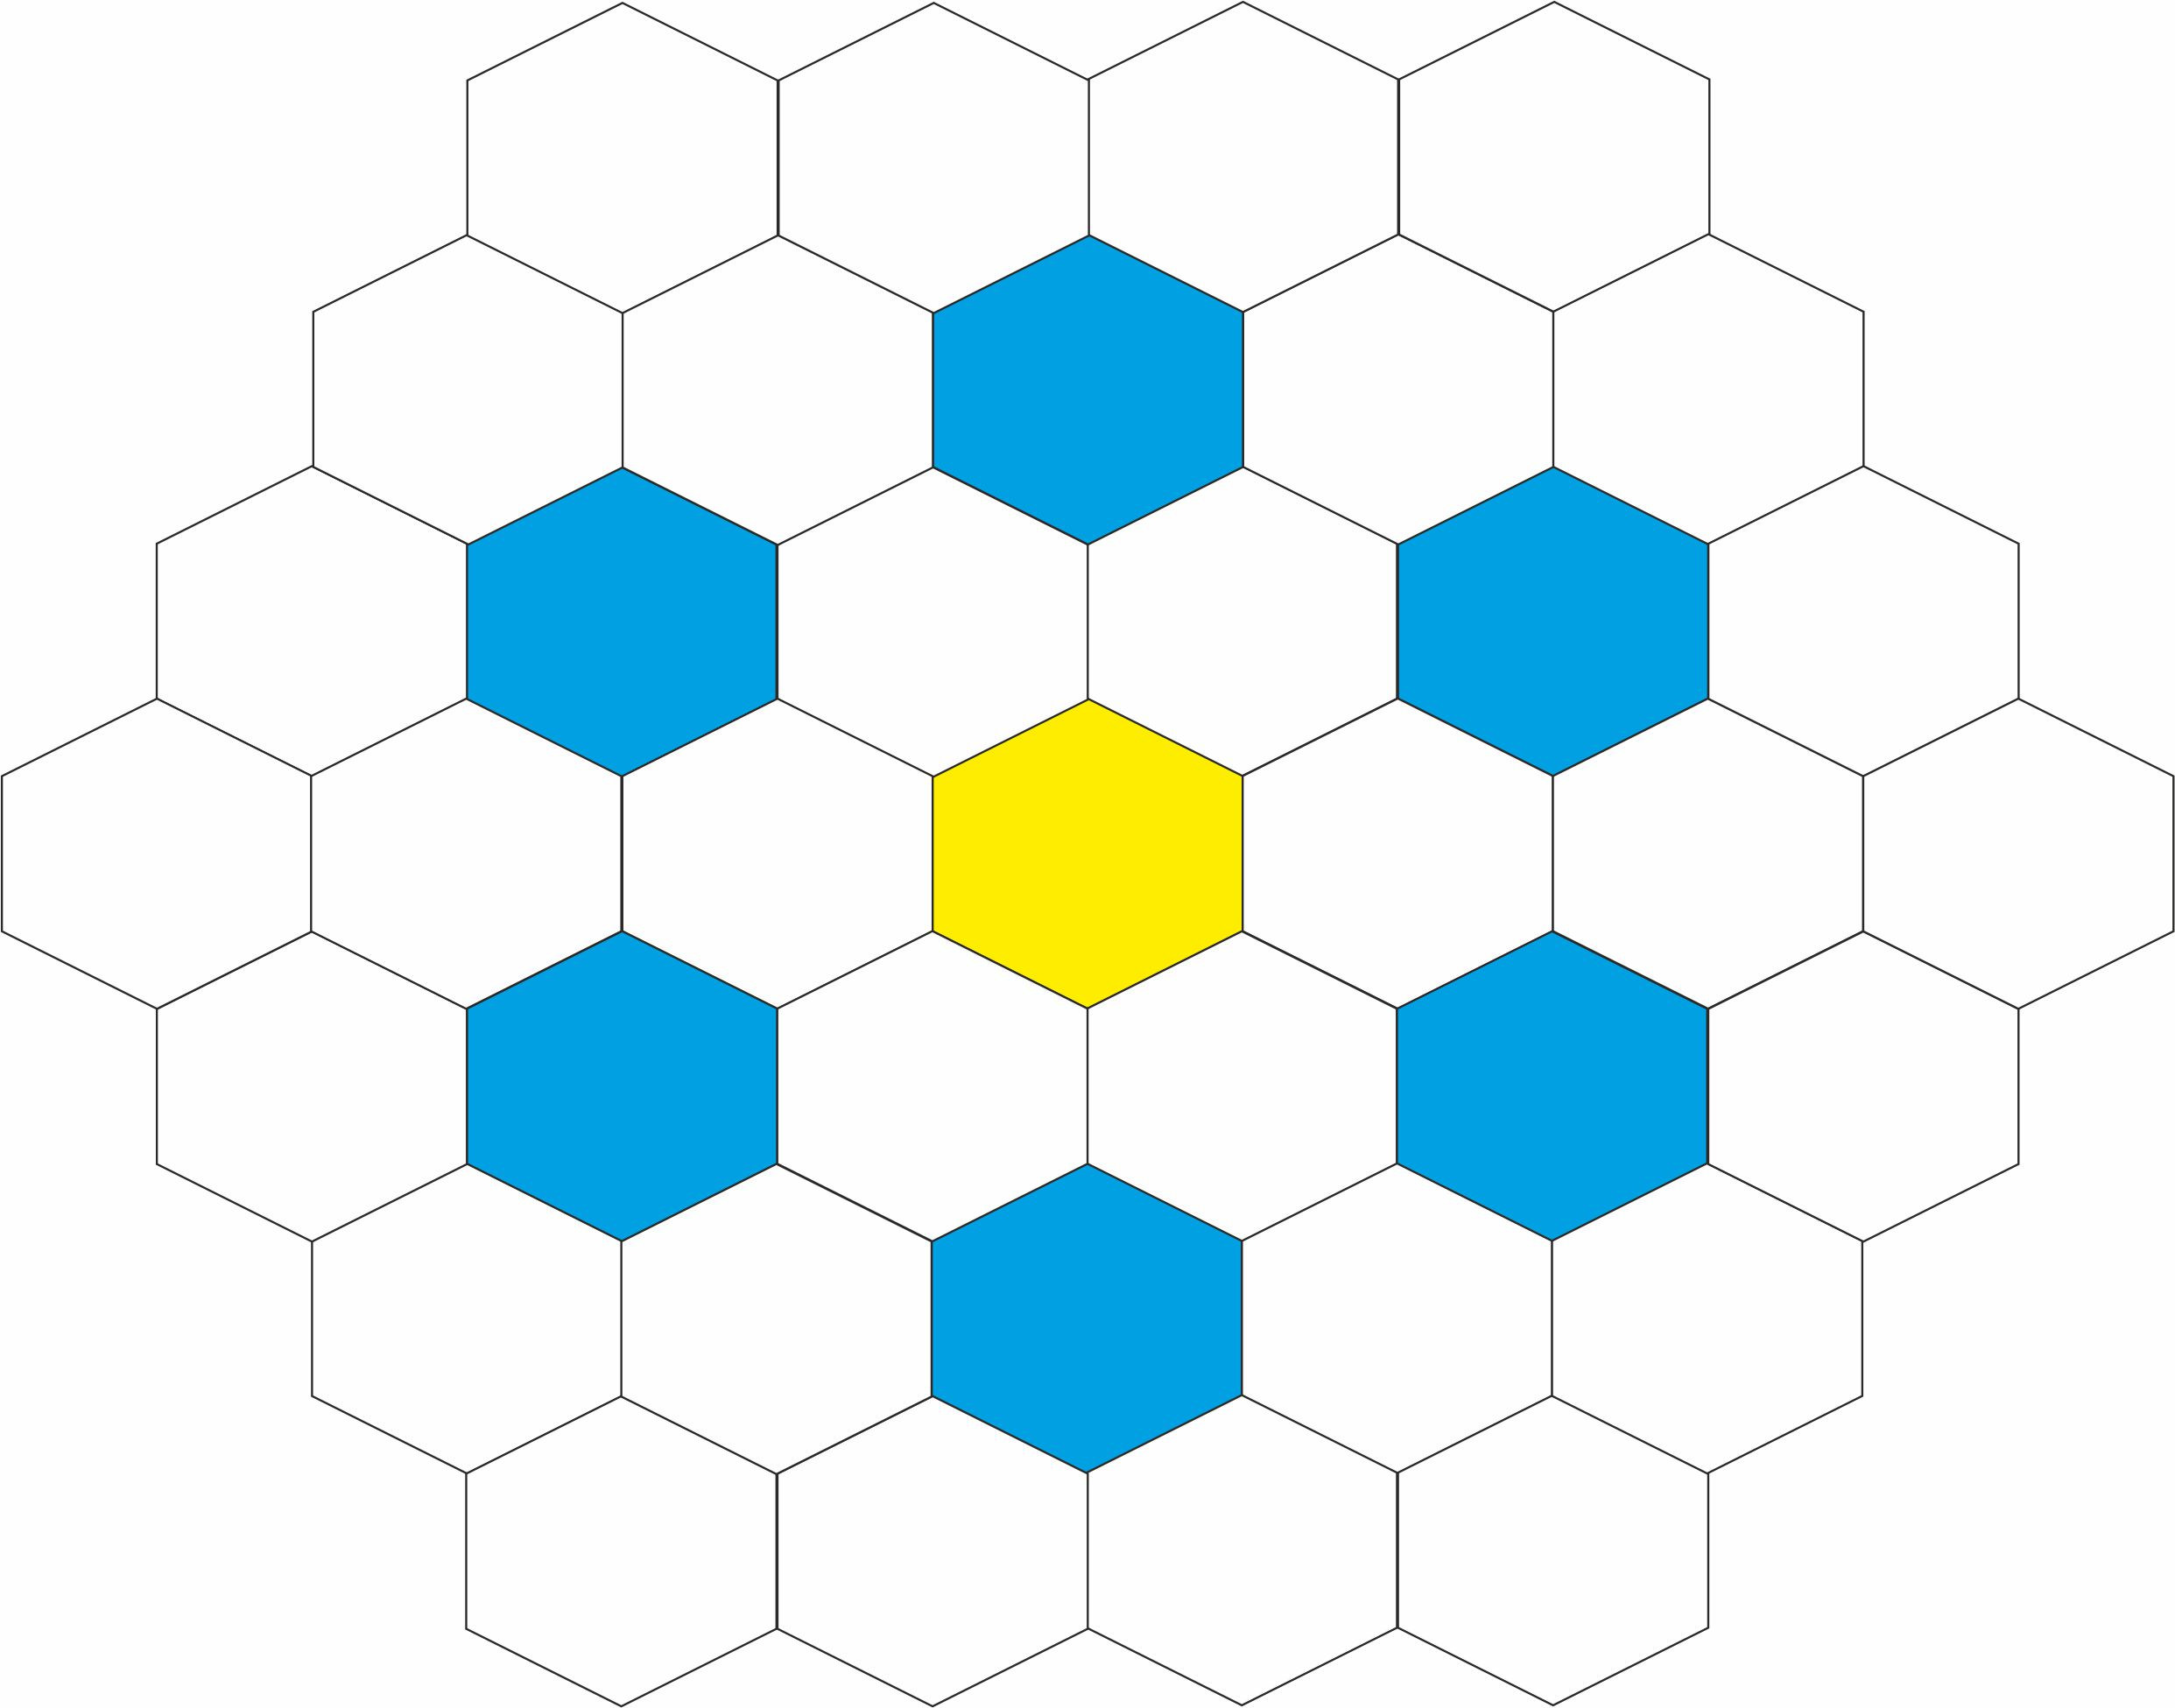
\includegraphics[scale=0.3]{kepek/Diagonals.jpg}
\caption{"Átlós" szomszédok hexagon háló esetén}
\label{fig:Diagonals}
\end{figure}

Ennek a számítási módja az alábbi kódrészben látható.
\begin{cpp}  
Diagonal[] diagonalDirections = 
{ 
   Diagonal(+2, -1, -1), Diagonal(+1, +1, -2), Diagonal(-1, +2, -1), 
   Diagonal(-2, +1, +1), Diagonal(-1, -1, +2), Diagonal(+1, -2, +1)
};

public Diagonal DiagonalNeighbor(Diagonal diagonal, int direction)
{
   return Diagonal
   (
      diagonal.x + diagonalDirections[direction].x, 
      diagonal.y + diagonalDirections[direction].y, 
      diagonal.z + diagonalDirections[direction].z
   );
}         
\end{cpp}

\bigskip

\textit{Tengelyes koordináta-rendszer} használata esetén is lehetséges az algoritmus használata.
